\setcounter{chapter}{1}
\chapter{ÉTUDE PRÉLIMINAIRE}
\minitoc %insert la minitoc
\graphicspath{{Chapitre2/figures/}}

%\DoPToC

%==============================================================================
\pagestyle{fancy}
\fancyhf{}
\fancyhead[R]{\bfseries\rightmark}
\fancyfoot[R]{\thepage}
\renewcommand{\headrulewidth}{0.5pt}
\renewcommand{\footrulewidth}{0pt}
\renewcommand{\chaptermark}[1]{\markboth{\MakeUppercase{\chaptername~\thechapter. #1 }}{}}
\renewcommand{\sectionmark}[1]{\markright{\thechapter.\thesection~ #1}}

\begin{spacing}{1.5}

%==============================================================================
\section*{Introduction}
Après avoir présenté le cadre général de notre projet et le cœur du sujet, nous entamons par le biais de ce chapitre une étude théorique, préface à sa réalisation. L'étude de l'existant sera l'opportunité de présenter plus en détail la problématique rencontrée. Une mise au point sur l'état des lieux de la gestion de projets du côté des clients de l'entreprise attestera de l'intérêt du projet pour un usage externe à l'entreprise. Enfin, une vue d'ensemble de solutions similaires présentes sur le marché permettra de se faire une idée globale sur les fonctionnalités à attendre du produit.


%==============================================================================
\section{Étude de l'existant}
L'étude de l'existant permet d'identifier les points forts ainsi que les points faibles de la démarche existante. Cette étude permettra de bien cibler les besoins de l'entreprise, en vue d'en tenir compte lors de la conception et du développement de la solution.
%-----------------------------------------------------------------------------------
\subsection{Description de l'existant}
La démarche de gestion de projet actuelle se base sur l'utilisation du logiciel Excel pour générer des documents associés aux différentes activités d'un projet. En effet, le chef de projet répertorie chaque catégorie d'artéfact associée à la gestion d'un projet sous forme de tableur Excel. Il procède ainsi à l'ajout et l'édition d'entrées pour chaque catégorie d'artéfact et y indique l'ensemble des informations requises. Cette procédure est facilitée par la duplication de fiches Excel de base, vierges, préparées à l'avance pour chaque catégorie. Ainsi, pour chaque catégorie d'artéfact; l'ensemble des entêtes et des valeurs prédéfinies pour chaque champs y est déja déclaré. La table d'entrées est accompagnée d'un ensemble d'indicateurs, statiques et dynamiques, pertinents à la catégorie en question. On y retrouve également les logos de l'entreprise IT SERV et du client porteur de projet. Des exemples de ces fiches sont exposés aux figures \ref{fig:risqueFiche} et \ref{fig:actionFiche}, traitant respectivement des artéfacts risques et actions pour un projet.

\begin{figure}[H]
\centering
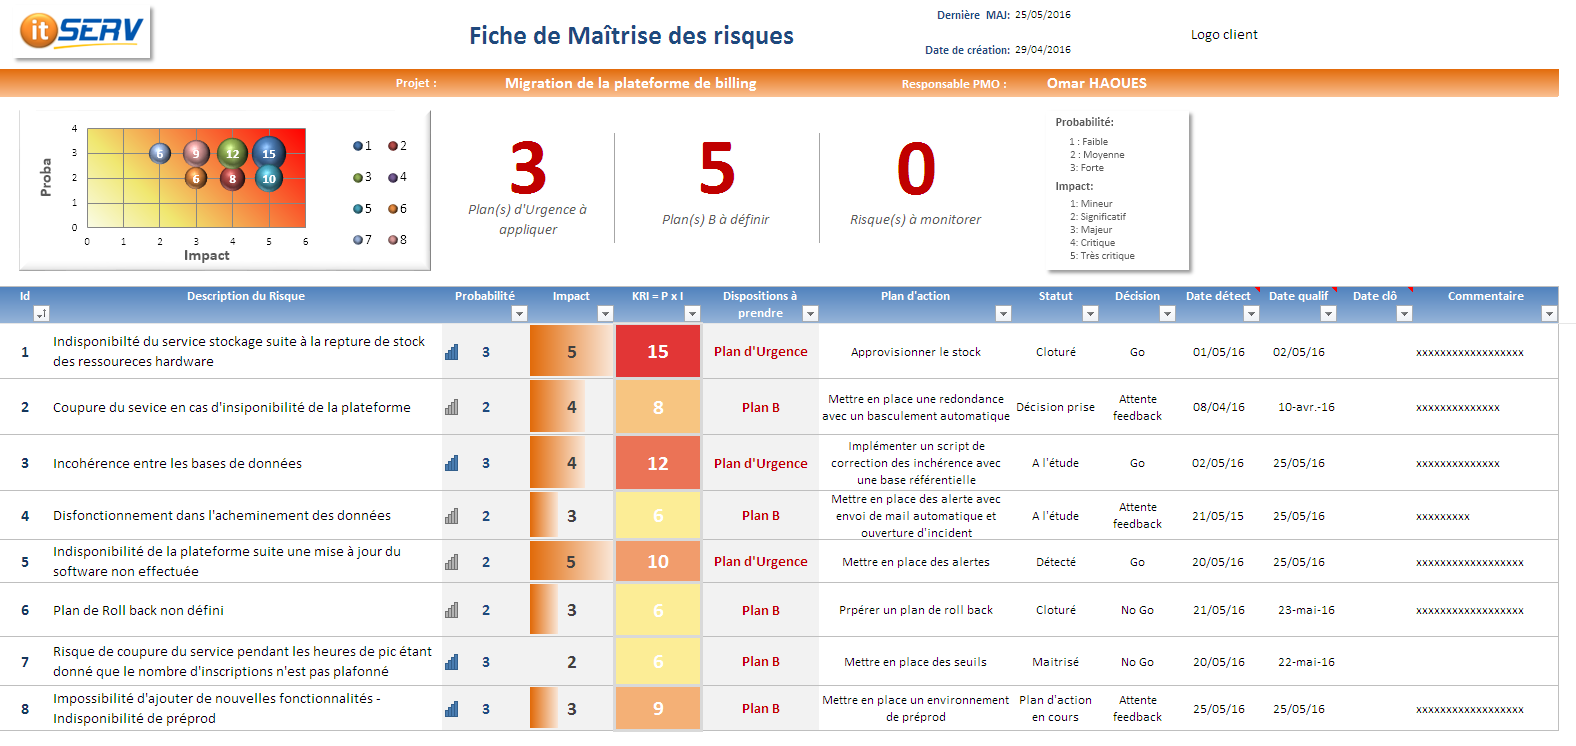
\includegraphics[width=\linewidth]{ficheRisques.png}
\caption{Exemple d'une fiche de maîtrise des risques}
\label{fig:risqueFiche}
\end{figure}

\begin{figure}[H]
\centering
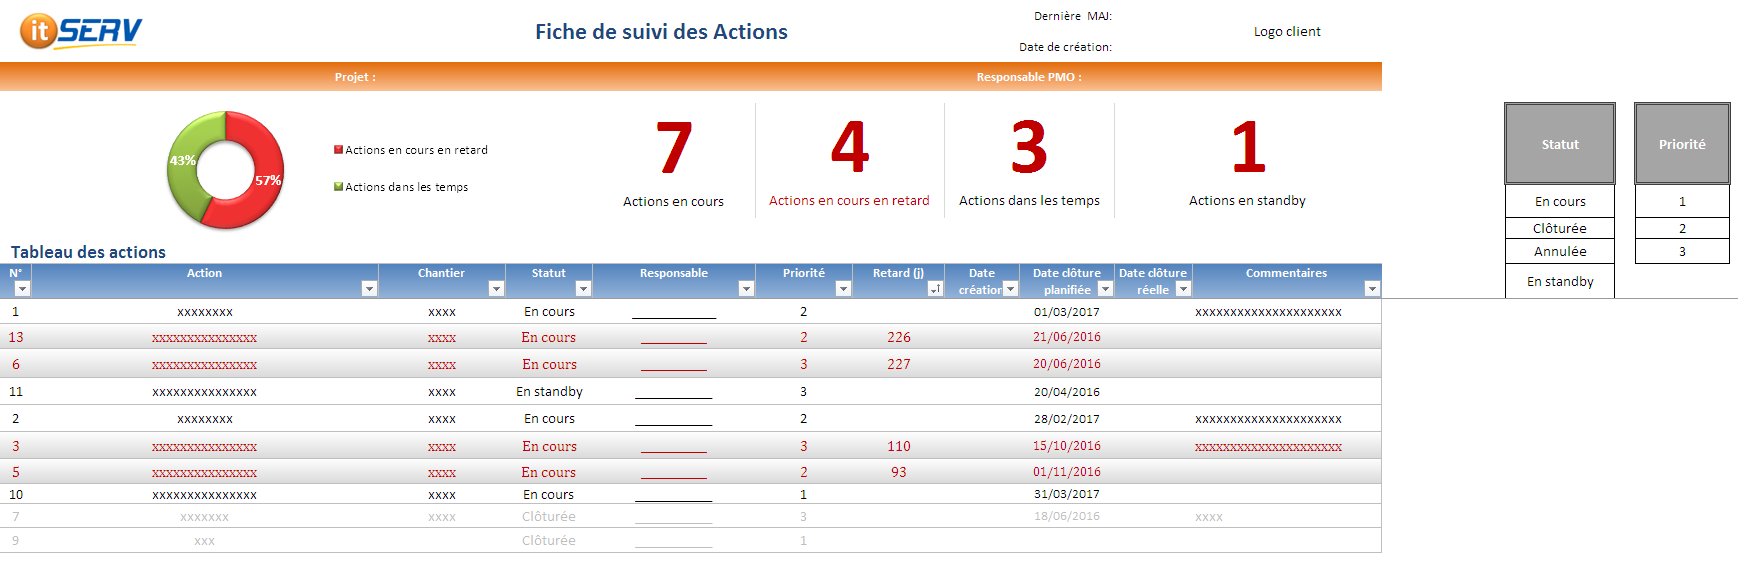
\includegraphics[width=\linewidth]{ficheActions.png}
\caption{Exemple d'une fiche de suivi des actions}
\label{fig:actionFiche}
\end{figure}
\

Le chef de projet est régulièrement chargé de diffuser les mises à jour relatives à un projet, périodiquement ou à la demande, au travers de l'envoi de messages électroniques directement aux parties concernées.\\

Cette méthode de travail possède certains atouts, mais dissimule dans l'ensemble plusieurs inconvenances qui nuisent à son niveau d'efficacité et à la performance de la gestion de projets par l'entreprise. Ces points sont exposés dans la section suivante.

%-----------------------------------------------------------------------------------
\subsection{Critique de l'existant}
La présentation de la méthode de gestion actuelle nous permet de déceler des limitations importantes, inhérentes à la démarche générale.\\
\\
Reconnaissons tout d'abord les mérites non négilgeables de celle-ci, à savoir :
\begin{itemize}
    \item Disponibilité de fiches de base, contraignant les champs à choix retraints aux options prédéfinies
    \item Présence de champs autocalculés ainsi que de supports visuels, assistant le client dans la compréhension de certains champs, dont la signification peut s'avérer obscure
    \item Génération automatique d'indicateurs riches (statistiques numériques, graphiques en camembert, ...)
\end{itemize}
\

Outre ces quelques bénéfices, cette méthode de gestion présente les nombreuses limitations suivantes :
\begin{itemize}
    \item \textbf{Perte en productivité} : induite d'un déficit d'automatisation de la démarche de gestion des fichiers
    \item \textbf{Fragmentation des données} : les données relatives à chaque projet sont réparties, sous forme d'une multitude de documents, souvent désorganisés
    \item \textbf{Journalisation non fiable des mises à jour} : la responsaibilité de celle-ci relève entièrement de l'oraganisation choisie par le chef de projet, et requiert un effort manuel, exclusivement dédié à la tâche
    \item \textbf{Traçabilité impossible} : l'origine des modifications des fichiers n'est pas connue
    \item \textbf{Stockage inneficace} : problème de centralisation pour de l'ensemble des données des projets menés par l'entreprise, redondance de données, oraganisation manuelle, ...
    \item \textbf{Sécurité non garantie} : la sécurisation des données est entièrement à la charge des parties prenantes y ayant accès
    \item \textbf{Condifentailité diffciele à assurer} : elle implique en pratique l'édition soigneuse, au cas par cas, des fichiers partagés
    \item \textbf{Synthèse des données impossible} : impossible de se reposer fiablement sur les données des fichiers pour les besoins d'aide à la décision de l'entreprise (dû aux problèmes susmentionnés)
    \item \textbf{Collaboration fastidieuse} : contribution d'intervenants non gérée par la solution actuelle. Le chef de projet transforme individuellement tous les flux d'information en données, avant de les indiquer dans le fichier approprié
\end{itemize}
\

Ce nombre abondant de limitations impose pour l'entreprise une révolution dans sa méthode actuelle de gestion de projets. Notre projet a pour but de fournir une solution adéquate à l'ensemble de ces lacunes. La solution à concevoir aspire ainsi à combiner les points forts de la démarche existante tout en apportant une solution efficace à ses problèmes inhérents.


%==============================================================================
\section{Étude des solutions existantes sur le marché}
Le problème de gestion de projet est aussi vieux que le concept de projet lui-même. En conséquence, un nombre important de solutions logicielles d'aide à la gestion de projet est disponible aujourd'hui sur le marché. Dans le but de produire une solution de qualité, une étude de l'existant s'impose afin de prendre en considération les points forts et les points faibles des solutions existantes. Celle-ci servira surtout à nous guider dans l'élaboration de la vision de notre produit.

%-----------------------------------------------------------------------------------
\subsection{Présentation des solutions existantes}
Les solutions présentes sur le marché se distinguent les unes des autres surtout par le niveau de fonctionnalités offert, et le domaine d'application cible. En effet, des solutions populaires, telle que JIRA \ref{JIRA}, se limitent à un domaine très particulier, en l'occurence la gestion de projets agiles pour cette dernière. Les solutions étudiées aspirent à être le plus générique possible, capable d'être employées dans n'importe quel contexte de projet. L'échantillon exposé ci-dessous vise à présenter une vue d'ensemble des caractéristiques communes et distinctives des solutions les plus populaires sur le marché, qui partagent cette vision.

\subsubsection*{MS Projects} %-------------------------------------------------------------------------
Microsoft Projects a su s'imposer pendant longtemps en tant que solution de facto pour les besoins de gestion de projet en entreprise. Faisant partie de la suite logicille de la firme, MS Projects ne fait pas exception et s'intègre pleinement à sa plateforme collaborative \ref{Office 365}, ce qui représente un réel bénéfice pour les clients ayant déja opté pour l'intégration de leurs données sur cette dernière. Le logiciel continue d'introduire un nombre de fonctionnalités avancées avec ses mises à jour. Ceci le rend particulièrement adapté aux besoins poussés de gestion de projet. Les utilisateurs expérimentés y trouvent leur compte, mais la courbe d'apprentisage est souvent pénible pour les utilisateurs novices et s'avère être trop complexe pour les usagers se limitant en besoin à un nombre restreint de ses fonctionnalités.

\subsubsection*{ProjectManager.com} %------------------------------------------------------------------
ProjectManager.com couvre très bien les fonctionnalités de base de gestion de projet et parmi toutes les solutions étudiées, s'apparente le plus à la vision initiale élaborée. Cette solution, disponible sous une offre SaaS \ref{SaaS}, s'adapte parfaitement aux besoins des petites et moyennes entreprises, qui retrouvent une simplicité d'usage associée à une couverture plus que décente des piliers de la gesion professionnel de projet.

\subsubsection*{Zoho Projects} %-----------------------------------------------------------------------
Zoho propose une suite logiceille qui répond aux besoins des particuilers et des entreprises. Dans cette optique, sa solution de gestion de projet s'intègre parfaitement avec qualques uns de ses autres produits, afin d'étendre ses fonctionnalités. La solution se veut simple, mais complète, en offrant un éventail éttoffé de fonctionnalités pour la gestion des divers facettes d'un projet. Elle se caractérise par une attention particuière apportée à l'ergonomie et au confort d'utilisation.

\subsubsection*{EasyProject} %-----------------------------------------------------------------------------
Redmine est la solution open source la plus complète disponible sur le marché. Cependant, son manque d'intuitivité et le faible niveau d'ergonomie offert, associés à son interface datée, nuisent à son potentiel et en font une solution peu courante d'usage dans la pratique. C'est tout d'abord dans le but d'accroître son utilisabilité, tout en prenant avantage de la base de fonctionnalités existante, que la solution EasyProject offre une version commerciale, basée sur cette solution. Depuis, la solution s'est vu évoluer vers l'une des solutions les plus abouties du marché.

\subsubsection*{Clarizen} %-----------------------------------------------------------------------------
Due à l'amélioration continue de son produit et à la complétude de sa vision, l'entreprise Clarizen a vu son produit se hisser à la position de Leader dans dans les classements Gartner et Forrester de 2016 \ref{clarizen.com} dans la catégorie de solutions SaaS de gestion de projets. De ce fait, ce produit a sans nul doute sa place dans notre étude, et impose une fine synthèse de ses traits caractéristiques qi lui valent son succès.
\\

Dans le but de présenter un échantillon pertinent de l'existant sur le marché, plusieurs solutions ont été omises, notamment pour des raisons de redondance ou de pauvreté en termes de fonctionnalités. Nous enchaînons avec la mise en relief des points communs et distinctifs de chacune dans la partie qui suit.

%-----------------------------------------------------------------------------------
\subsection{Critique des solutions existantes}

\subsubsection*{Points communs} %-----------------------------------------------------------------------------
Les solutions retenues partagent un tronc commun de fonctionnalités destinées à la gestion des aspects cruciaux d'un projet, primordialement :

\begin{itemize}
    \item \textbf{La plannification} :
%    \item \textbf{} :
\end{itemize}
\


\subsubsection*{Points distinctifs} %-----------------------------------------------------------------------------

\begin{table}[h]
\centering
\begin{tabular}{|l|1|1|1|l|1|}
\hline
% after \\: \hline or \cline{col1-col2} \cline{col3-col4} ...
        Caractéristiques & MS Projects & P.M .com & Zoho Projects & EasyProject & Clarizen\\
\hline
        Type & Bureau \& Local* & SaaS & SaaS & SaaS \& Local & SaaS\\

\hline
        Workflow & & & & & \\


\hline
        WBS ✓ & & & & ✓ & \\
\hline
        Diagramme de Gantt & ✓ & ✓ & ✓ & ✓ & ✓ \\
\hline
        Reporting & ✓ & ✓ & ✓ & ✓ & ✓ \\
\hline
        Jalonnage & & & & ✓ & \\
\hline
        Gestion budget & & & & & \\
\hline
        Gestion des charges & & & & & \\
\hline
        Gestion des risques & & & & & \\
\hline
        Gestion de l'avancement & & & & & \\
\hline
        Niveaux projet & & & & & \\
\hline
        Workflow & & & & & \\
\hline
        GED & & & & & \\
\hline
        Terminaux mobiles & (Web? & )App & & & & \\
\hline
        Intégration & & & Slack, ... & & \\
\hline
        Standardisation PMP & & & & ✓ & \\
\hline
        Gestion du portfolio & & & & & \\
\hline
\end{tabular}
\caption{Comparatif des solutions de gestion de projet présentées}
\label{comparatifSolutionsEtudiees}

\end{table}


Cependant, vu son expertise en développement d'applications, IT SERV a choisi de développer son propre logiciel d'aide à la gestion de projet.

%==============================================================================
\section*{Conclusion}


%==============================================================================
\end{spacing}
